\chapter{Introduction}

In this introductory chapter, we make an overview of simplex-based algorithms.
We present the main features of the \scifunction{neldermead} component, and 
show how to use the component with a simple example.

\section{Overview}
\index{Torczon, Virginia}
\index{Wright, Margaret}

The Nelder-Mead simplex algorithm \cite{citeulike:3009487}, published in 1965, is an enormously 
popular search method for multidimensional unconstrained optimization. 
The Nelder-Mead algorithm should not be confused with the (probably) 
more famous simplex algorithm of Dantzig for linear programming. The 
Nelder-Mead algorithm is especially popular in the fields of chemistry, 
chemical engineering, and medicine. Two measures of the ubiquity of the 
Nelder-Mead algorithm are that it appears in the best-selling handbook 
Numerical Recipes and in Matlab. In \cite{Torczon89multi-directionalsearch},
Virginia Torczon writes: "Margaret Wright has stated that over
fifty percent of the calls received by the support group for the NAG
software library concerned the version of the Nelder-Mead 
simplex algorithm to be found in that library". No derivative of the cost function is 
required, which makes the algorithm interesting for noisy problems.

The Nelder-Mead algorithm falls in the more general class of direct 
search algorithms. These methods use values of $f$ taken from a set of 
sample points and use that information to continue the sampling. The 
Nelder-Mead algorithm maintains a simplex which are approximations of an 
optimal point. The vertices are sorted according to the objective 
function values. The algorithm attemps to replace the worst vertex with 
a new point, which depends on the worst point and the centre of the best 
vertices. 

The goal of this toolbox is to provide a Nelder-Mead (1965) direct search optimization method to solve the 
following unconstrained optimization problem
\begin{eqnarray}
\min f(\bx)
\end{eqnarray}
where $\bx\in \RR^n$, $n$ is the number of optimization parameters and $f$ is the objective 
function $f:\RR^n\rightarrow \RR$.
In order to solve the unconstrained optimization problem, the Nelder-Mead 
algorithm uses a variable shape simplex. The toolbox also provide Spendley's et al. 
algorithm \cite{Spendley1962} (1962), which uses a fixed shape simplex. Historically, the algorithm created  
by Nelder and Mead was designed as an improvement on Spendley's et al. algorithm.
The Box complex algorithm \cite{Box1965} (1965), which is an extension of Spendley's  et al. algorithm, solves the 
following constrained problem
\begin{eqnarray}
&&\min f(\bx)\\
&&\ell_i \leq x_i \leq u_i, \qquad i = 1,n\\
&&g_j(\bx)\geq 0, \qquad j = 1, m\\
\end{eqnarray}
where $m$ is the number of nonlinear, positive constraints and $\ell_i,u_i\in \RR^n$ are the lower 
and upper bounds of the variables.

The Nelder-Mead algorithm may be used in the following optimization context :
\begin{itemize}
\item there is no need to provide the derivatives of the objective function,
\item the number of parameters is small (up to 10-20),
\item there are bounds and/or non linear constraints.
\end{itemize}

The internal design of the system is based on the following components.
\begin{itemize}
\item The "neldermead" component provides various simplex-based 
algorithms and manages for Nelder-Mead specific settings, such as the 
method to compute the initial simplex and the specific termination 
criteria.
\item The "fminsearch" component provides a Scilab commands which aims 
at behaving as Matlab's fminsearch. Specific terminations criteria, 
initial simplex and auxiliary settings are automatically configured so 
that the behavior of Matlab's fminsearch is exactly reproduced.
\item The "optimset" and "optimget" components provide Scilab commands 
to emulate their Matlab counterparts.
\item The "nmplot" component provides features to 
produce directly output pictures for Nelder-Mead algorithm.
\end{itemize}
The current toolbox is based on (and therefore requires) the following components.
\begin{itemize}
\item The "optimbase" component provides an abstract class for a general optimization 
component, including the number of variables, the minimum and maximum 
bounds, the number of non linear inequality constraints, the logging 
system, various termination criteria, the cost function, etc...
\item The "optimsimplex" component provides a class to manage a simplex made of an 
arbitrary number of vertices, including the computation of a simplex by 
various methods (axes, regular, Pfeffer's, randomized bounds), the 
computation of the size by various methods (diameter, sigma +, sigma-, 
etc...) and many algorithms to perform reflections and shrinkages.
\end{itemize}

The following is a list of features the Nelder-Mead algorithm currently provides :
\begin{itemize}
\item manage various simplex initializations
  \begin{itemize}
  \item initial simplex given by user,
  \item initial simplex computed with a length and along the coordinate axes,
  \item initial regular simplex computed with Spendley et al. formula
  \item initial simplex computed by a small perturbation around the initial guess point
  \end{itemize}
\item manage cost function
  \begin{itemize}
  \item optionnal additionnal argument
  \item direct communication of the task to perform : cost function or inequality constraints
  \end{itemize}
\item manage various termination criteria 
  \begin{itemize}
  \item maximum number of iterations, 
  \item tolerance on function value (relative or absolute),
  \item tolerance on x (relative or absolute),
  \item tolerance on standard deviation of function value (original termination criteria in [3]),
  \item maximum number of evaluations of cost function,
  \item absolute or relative simplex size,
  \end{itemize}
\item manage the history of the convergence, including :
  \begin{itemize}
  \item the history of function values,
  \item the history of optimum point,
  \item the history of simplices,
  \item the history of termination criterias,
  \end{itemize}
\item provide a plot command which allows to graphically see the history of the simplices toward the optimum,
\item provide query functions for 
  \begin{itemize}
  \item the status of the optimization process,
  \item the number of iterations, 
  \item the number of function evaluations, 
  \item the status of execution, 
  \item the function value at initial point, 
  \item the function value at optimal point, 
  \item etc...
  \end{itemize}
\item Spendley et al. fixed shaped algorithm,
\item Kelley restart based on simplex gradient,
\item O'Neill restart based on factorial search around optimum,
\item Box-like method managing bounds and nonlinear inequality constraints based on arbitrary number of vertices in the simplex.
\end{itemize}

\section{How to use the Toolbox}

The design of the toolbox is based on the creation of 
a new token by the \scifunction{neldermead\_new} function.
The Nelder-Mead object associated with this token can then 
be configured with \scifunction{neldermead\_configure} and queried 
with \scifunction{neldermead\_cget}. For example, the
\scifunction{neldermead\_configure} command allows to configure the 
number of variables, the objective function and the initial guess.

The main command of the toolbox is the \scifunction{neldermead\_search} command, which
solves the optimization problem. After an optimization has been performed,
the \scifunction{neldermead\_get} command allows to retrieve the optimum $x^\star$,
as well as other parameters, such as the number of iterations performed, the number 
of evaluations of the function, etc...

Once the optimization is finished, the \scifunction{neldermead\_destroy} function 
deletes the object.

\section{An example}

In the following example, we search the minimum of the 2D Rosenbrock function \cite{citeulike:1903787}, 
defined by
\begin{eqnarray}
f(x_1,x_2) = 100(x_2 - x_1)^2 + (1-x_1)^2
\end{eqnarray}

The following Scilab script allows to find the solution of the problem. 
We begin by defining the function \scifunction{rosenbrock} which computes the Rosenbrock function. 
The traditionnal initial guess $(-1.2 , 1.0)$ is used, which corresponds 
to the "-x0" key. The initial simplex is computed along 
the axes with a length equal to 0.1. We want to use the Nelder-Mead algorithm with variable simplex size 
is used, which corresponds to the "variable" value of the "-method" option. 
The verbose mode is enabled so that messages are generated during the algorithm. 
After the optimization is performed, the optimum is retrieved with quiery features.

\lstset{language=scilabscript}
\begin{lstlisting}
function y = rosenbrock (x)
  y = 100*(x(2)-x(1)^2)^2 + (1-x(1))^2;
endfunction
nm = neldermead_new ();
nm = neldermead_configure(nm,"-numberofvariables",2);
nm = neldermead_configure(nm,"-x0",[-1.2 1.0]');
nm = neldermead_configure(nm,"-simplex0method","axes");
nm = neldermead_configure(nm,"-simplex0length",0.1);
nm = neldermead_configure(nm,"-method","variable");
nm = neldermead_configure(nm,"-verbose",1);
nm = neldermead_configure(nm,"-function",rosenbrock);
nm = neldermead_search(nm);
xopt = neldermead_get(nm,"-xopt")
fopt = neldermead_get(nm,"-fopt")
status = neldermead_get(nm,"-status")
nm = neldermead_destroy(nm);
\end{lstlisting}

This produces the following output.

\lstset{language=scilabscript}
\begin{lstlisting}
-->nm = neldermead_search(nm);
Function Evaluation #1 is [24.2] at [-1.2 1]
Function Evaluation #1 is [24.2] at [-1.2 1]
Function Evaluation #2 is [8.82] at [-1.1 1]
Function Evaluation #3 is [16.4] at [-1.2 1.1]
Step #1 : order
=================================================================
Iteration #1 (total = 1)
Function Eval #3
Xopt : -1.1 1
Fopt : 8.820000e+000
DeltaFv : 1.538000e+001
Center : -1.1666667 1.0333333
Size : 1.414214e-001
Vertex #1/3 : fv=8.820000e+000, x=-1.100000e+000 1.000000e+000
Vertex #2/3 : fv=1.640000e+001, x=-1.200000e+000 1.100000e+000
Vertex #3/3 : fv=2.420000e+001, x=-1.200000e+000 1.000000e+000
Reflect
xbar=-1.15 1.05
Function Evaluation #4 is [5.62] at [-1.1 1.1]
xr=[-1.1 1.1], f(xr)=5.620000
Expand
Function Evaluation #5 is [4.428125] at [-1.05 1.15]
xe=-1.05 1.15, f(xe)=4.428125
  > Perform Expansion
Sort
[...]
=================================================================
Iteration #56 (total = 56)
Function Eval #98
Xopt : 0.6537880 0.4402918
Fopt : 1.363828e-001
DeltaFv : 1.309875e-002
Center : 0.6788120 0.4503999
Size : 6.945988e-002
Vertex #1/3 : fv=1.363828e-001, x=6.537880e-001 4.402918e-001
Vertex #2/3 : fv=1.474625e-001, x=7.107987e-001 4.799712e-001
Vertex #3/3 : fv=1.494816e-001, x=6.718493e-001 4.309367e-001
Reflect
xbar=0.6822933 0.4601315
Function Evaluation #99 is [0.1033237] at [0.6927374 0.4893262]
xr=[0.6927374 0.4893262], f(xr)=0.103324
Expand
Function Evaluation #100 is [0.1459740] at [0.7031815 0.5185210]
xe=0.7031815 0.5185210, f(xe)=0.145974
  > Perform reflection
Sort
=================================================================
Iteration #57 (total = 57)
Function Eval #100
Xopt : 0.6927374 0.4893262
Fopt : 1.033237e-001
DeltaFv : 4.413878e-002
Center : 0.6857747 0.4698631
Size : 6.262139e-002
Vertex #1/3 : fv=1.033237e-001, x=6.927374e-001 4.893262e-001
Vertex #2/3 : fv=1.363828e-001, x=6.537880e-001 4.402918e-001
Vertex #3/3 : fv=1.474625e-001, x=7.107987e-001 4.799712e-001
Terminate with status : maxfuneval
-->xopt = neldermead_get(nm,"-xopt")
 xopt  =
 
    0.6927374  
    0.4893262  
 
-->fopt = neldermead_get(nm,"-fopt")
 fopt  =
 
    0.1033237  
 
-->status = neldermead_get(nm,"-status")
 status  =
 
 maxfuneval   
\end{lstlisting}

\section{Help, demonstrations and unit tests}

For a complete presentation of the functions and options, the reader 
should consult the help which is provided with the component.
The main menu of the help associated with the optimization 
module is presented in figures \ref{fig-intro-help} and \ref{fig-intro-helpfminsearch}.
The corresponding pages provide a complete documentation for the 
corresponding functions, as well as many sample uses.

\begin{figure}
\begin{center}
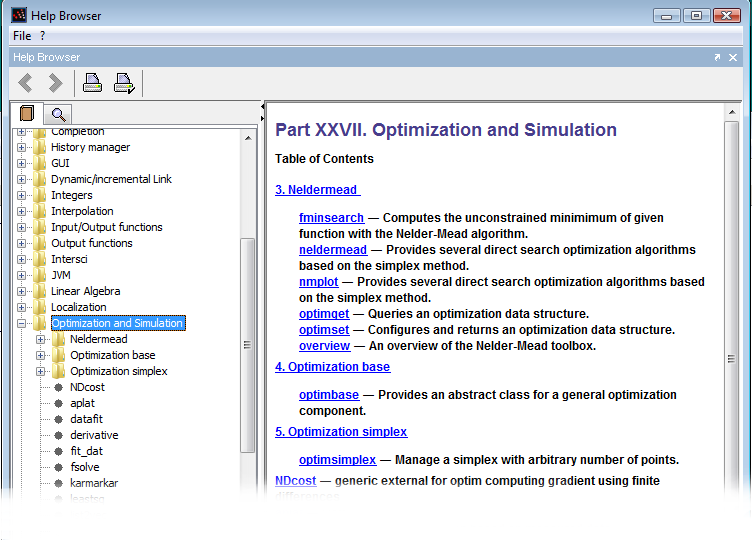
\includegraphics[width=15cm]{introduction-help.png}
\end{center}
\caption{Built-in help for the Nelder-Mead component}
\label{fig-intro-help}
\end{figure}

\begin{figure}
\begin{center}
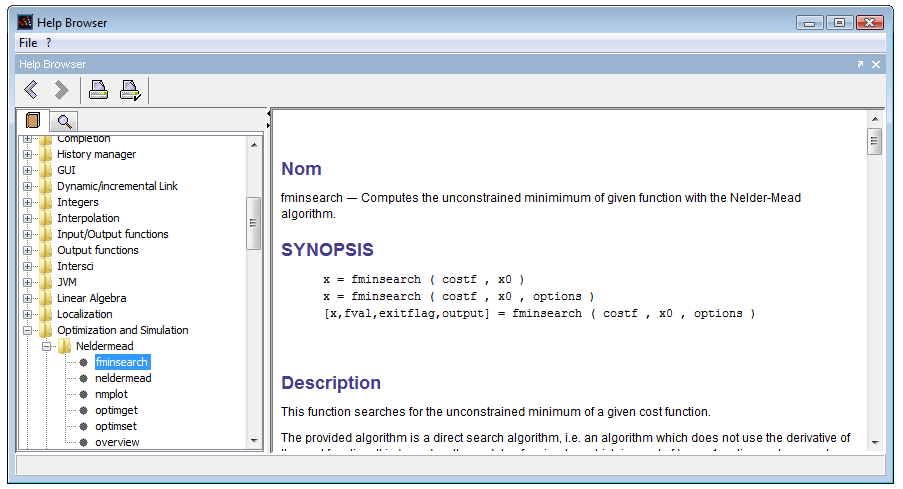
\includegraphics[width=15cm]{introduction-help-fminsearch.png}
\end{center}
\caption{Built-in help for the \scifunction{fminsearch} function}
\label{fig-intro-helpfminsearch}
\end{figure}

Several demonstrations are provided with the component. These 
are available from the "Demonstration" menu of the Scilab console
and are presented in figure \ref{fig-intro-demos}.

\begin{figure}
\begin{center}
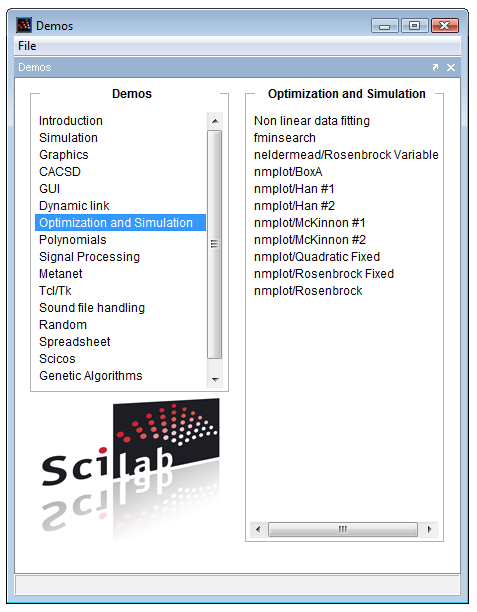
\includegraphics[width=10cm]{introduction-demos.png}
\end{center}
\caption{Built-in demonstration scripts for the Nelder-Mead component}
\label{fig-intro-demos}
\end{figure}

The following script shows where the demonstration scripts are 
available from the Scilab installation directory.

\lstset{language=scilabscript}
\begin{lstlisting}
-->cd SCI/modules/optimization/demos/neldermead
 ans  =
 
 D:\Programs\SCFD8E~1\modules\optimization\demos\neldermead   
 
-->ls *.sce
 ans  =
 
!nmplot_rosenbrock.sce        !
!                             !
!nmplot_rosenbrock.fixed.sce  !
!                             !
!nmplot_quadratic.fixed.sce   !
!                             !
!nmplot_mckinnon2.sce         !
!                             !
!nmplot_mckinnon.sce          !
!                             !
!nmplot_han2.sce              !
!                             !
!nmplot_han1.sce              !
!                             !
!nmplot_boxproblemA.sce       !
!                             !
!neldermead_rosenbrock.sce    !
!                             !
!neldermead.dem.sce           !
!                             !
!fminsearch.sce               !
\end{lstlisting}

These components were developped based on unit tests, which are 
provided with Scilab.
These unit tests are located in the "SCI/modules/optimization/tests/unit\_tests"
directory, under the "neldermead", "optimsimplex" and "optimbase" directories.
Each unit test correspond to a .tst file. These tests are covering most 
(if not all) the features provided by the components. This is why there are 
a good source of information on how to use the functions.




